% Capítulo 4
\chapter{Projeto e implementação do \textit{Walking gait}}
\label{ch:Math}

\begin{guide}
	Detalhar implementação do walking gait
\end{guide}

\begin{guide}
	Detalhar matemática dos movimentos.
\end{guide}

\section{\textit{Walking gait}}

Nesta seção detalhes arquiteturais da implementação do \textit{walking gait} serão descritos.

O \textit{walking gait} é o componente que coordena a caminhada mantendo o estado drobô, sabendo onde cada perna encontra-se e o seu estágio durante a caminhada. Desta forma, quando algum evento de perturbação, ou de ajuste, é disparado o \textit{walking gait} inicia a atualização das juntas a partir do estado atual. Assim, podemos descrever a caminhada como um evento contínuo no tempo.

Para realizar a tarefa de forma adequada, o componente faz uso de multi-processamento. Três \textit{threads} dentro do componente são responsáveis por tarefas específicas essenciais ao complemento do comportamento geral da caminhada: A \textit{thread} de rede, a \textit{thread} atualização dos motores e a \textit{thread} principal.

\subsection{\textit{Thread} principal: Da geração da trajetória até a aplicação às juntas}

\begin{figure}[h!]
	\centering
	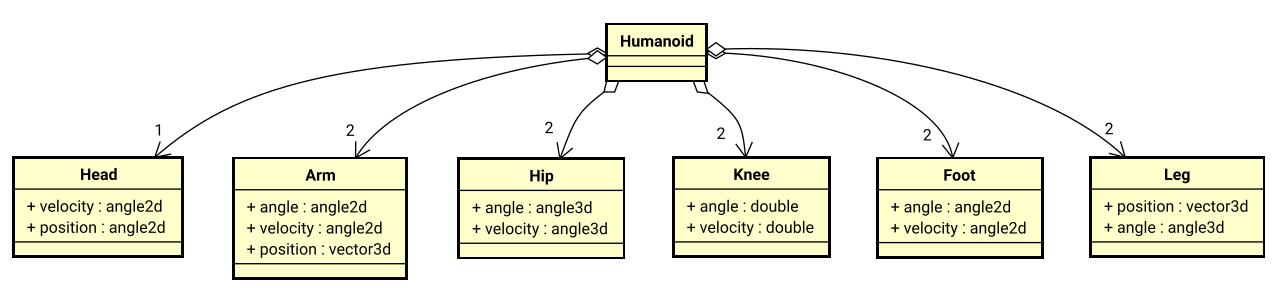
\includegraphics[scale=0.4]{imagens/svg/walkinggait-domain}
	\caption{Diagrama de domínio do \textit{walking gait}.}
	\label{fig:walkinggait:domain}
\end{figure}

A figura~\ref{fig:walkinggait:domain} mostra o diagrama de domínio das classes relevantes aos dados que o componente manipula. Nela podemos ver a classe $Humanoid$ é uma agregação de diversas outras classes que representam cada parte de Arash. É possível também observar que nas classes $Head$, $Arm$, $Hip$, $Knee$, $Foot$ existem dados ângulo e velocidade. Isso se dá por causa que componente utiliza essas informações para calcular o próximo estado do sistema em caso de algum distúrbio. Nota-se também, que a classe $Leg$ aparece de forma ambígua, já que existem as definições de $Hip$, $Knee$ e $Foot$. Porém, a classe $Leg$, representa os dados da cinemática inversa de uma perna, enquanto as demais classes guardam o estado atual das partes que representam.

Nota-se, também, a notação dos dados utilizados: $angle2d$, $angle3d$ e $vector3d$. Note que todos os tipos possuem o sufixo numérico, que indica a quantidade de dimensões aquela classe guarda, e a letra, que indica o tipo de seus dados, no caso $d$ que significa $double$. Para ângulos, $2$ dimensões significa que as dimensões $pitch$ e $roll$ são guardadas; já para $3$ dimensões as orientações $roll$, $pitch$ e $yaw$ são guardadas. Para vetores, os valores $x$, $y$ e $z$ são guardados.



\subsection{Servidor de controle}

A \textit{thread} de rede roda um servidor \textit{UDP} que aceita objetos serializandos em \textit{JSON} contendo informações de controle.




\section{Seção 1}
\label{sec:Orientacao}

Teste para símbolo

\simb[$\lambda$ (algum símbolo)]{$\lambda$}


\section{Seção 2}

Teste para abreviatura 

\abrv[IFRN -- Instituto Federal do Rio Grande do Norte]{IFRN}

\abrv[DIATINF -- Diretoria Acadêmica de Gestão e Tecnologia da
Informação]{DIATINF}
